\chapter[Metodología de Trabajo]{Metodología de Trabajo}
\label{cp:methodology}

\parindent0pt


Para llevar a cabo los objetivos propuestos en este trabajo final es necesario definir una metodología consistente que permita planificar y gestionar las diferentes tareas y recursos de manera ordenada. Este capítulo detalla la planificación del plan de trabajo y el desgloce de actividades a través de las cuales se pretende llegar a obtener resultados (Sección \ref{thesis-plan}). Luego se describe la metodología de investigación elegida para el estudio del estado del arte del reciclado de vidrio y la adopción de tecnología blockchain (Sección \ref{sec:research-method}). Finalmente, se describe la metodología de desarrollo del prototipo tecnológico, comprendiendo las etapas de análisis de requerimientos, diseño, implementación, pruebas y despliegue (Sección \ref{sec:software-method}).

\section{Planificación del Plan de Trabajo}
\label{thesis-plan}

En esta sección se describen todos los pasos establecidos como parte del proceso necesario para desarrollar el prototipo basado en blockchain orientado a la trazabilidad y valorización del vidrio. En la Figura \ref{fig:activities-plan} se pueden observar las actividades que conforman el plan de trabajo para cumplir este objetivo. En primer lugar, comienza la formación (Actividad A) estudiando las bases de blockchain y los lenguajes de desarrollo asociados a este para poder discernir aquellas herramientas tecnológicas que sean más adecuadas para el desarrollo del software propuesto. Conforme avance el tiempo del trabajo final de grado se investigan los pormenores del reciclado, en particular, en el contexto regional de Mendoza (Actividad B). Una vez analizado el estado del arte y las tecnologías asociadas, se selecciona la metodología de trabajo que mejor se adapte a proceso de desarrollar software enfocado en trazabilidad y teniendo en cuenta las características únicas de utilizar blockchain (Actividad C). El proceso de desarrollo de software para una aplicación de trazabilidad sigue una serie de etapas planificadas y estructuradas para asegurar que el producto final cumple con los requisitos y necesidades del cliente, como cualquier otro software, por ende es necesario cumplimentar la serie de etapas previamente definidas en la Actividad C. Luego de selecciona la metodología, se dedica un periodo de tiempo exclusivamente a las actividades relacionadas con el desarrollo de la aplicación prototipo (Actividad D): análisis de requisitos, diseño del sistema, implementación de los requerimientos, pruebas y validación y finalmente reimplementación si fuera necesario hasta alcanzar el despliegue final. Todo el proceso anteriormente descripto puede llegar a pasar por diferentes iteraciones de progreso si fuera necesario. Finalmente, este trabajo concluye con la escritura del documento final de tesina donde se registra el proceso ejecutado y los resultados alcanzados (Actividad E).

\begin{itemize}
	\item \textbf{Actividad A}: completar la formación en blockchain y las tecnologías y plataformas relacionadas.
	\item \textbf{Actividad B}: realizar un estudio pormenorizado del estado actual del arte en todo lo relacionado con blockchain en el campo del reciclado. En particular, se orienta la búsqueda al reciclado de vidrio. Se analizan trabajos de la literatura como también aplicaciones blockchain orientadas al tema (si estas existen).
	\item \textbf{Actividad C}: definir los procesos de desarrollo del prototipo, haciendo hincapié en seguir los fundamentos de la ingeniería de software y planificando de forma concisa y clara.
	\item \textbf{Actividad D}: desarrollar la aplicación prototipo. Este desarrollo a su vez involucra las diferentes etapas de un proceso de desarrollo de software, desde análisis de requerimientos, diseño, implementación, evaluación, corrección del prototipo y despliegue. Todos estos pasos se aplican siguiendo una metodología específica, teniendo en cuenta las características particulares del sistema y que además permite llevar a cabo el objetivo general.
	\item \textbf{Actividad E}: Documentar en una memoria el proceso y resultados del trabajo realizado.
\end{itemize}

\begin{figure}[!htpb]
    \centering
    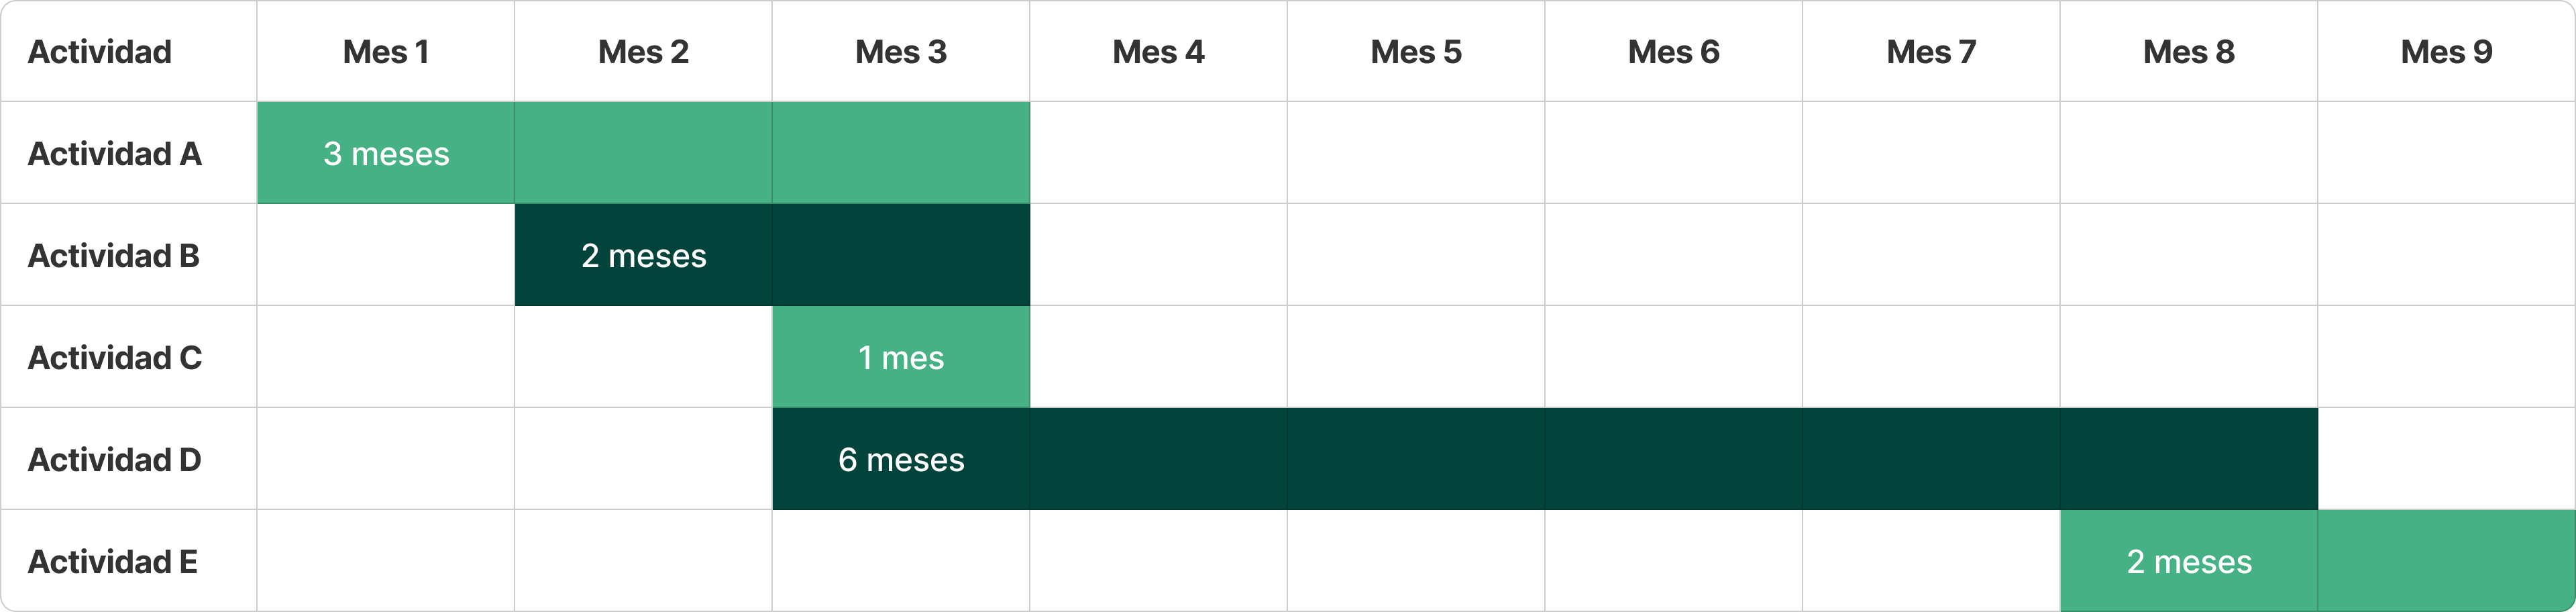
\includegraphics[width=0.8\textwidth]{Figures/activities-plan.png}
    \caption{Planificación de las actividades del plan de trabajo}
    \label{fig:activities-plan}
\end{figure}

En la Sección \ref{research-method} se detalla la metodología de investigación para llevar a cabo la Actividad B de estudio del estado del arte. Luego, en la Sección \ref{software-method} se describe la metodología de trabajo elegida para el proceso de desarrollo del prototipo tecnológico.

\section{Metodología de Investigación}
\label{sec:research-method}


En primer lugar, es necesario entender ...

Contar sobre la metodología de investigación del estado del arte, los viajes y las entrevistas.

\section{Metodología de Desarrollo}
\label{sec:software-method}

Hacer la comparación de metodologías de desarrollo y contar sobre la metodología en V elegida por qué la elegimos y describirla un poco. Poner figura de metodología en V.

Contar en qué etapa de la metodología hacemos:

Elección de herramientas, frameworks y softwares

Análisis de requerimientos

Implementación

Y cómo se lleva a cabo el testeo

Explicar que la documentación del proceso se fue realizando continuamente y se armó el informe al final a partir de toda la información registrada durante el proceso.

Explicar que trackeamos incidencias en Jira y que trackeamos evolución del código con git.
